\chapter{Proposed tridiagonal algorithm}

\section{Modified cyclic reduction for near-Toeplitz systems}

Here, we explore the idea of
exploiting the relatively simple matrix structure
of the coefficient matrix appearing in
tridiagonal compact finite difference schemes.
The coefficient matrix $A$ for tridiagonal schemes
has the following general form:

\begin{equation} \label{eqn:toeplitz-matrix}
A = 
\begin{pmatrix}
     b_1 & c_1  \\
     a_0 & b_0  &  c_0  \\
         & a_0  &  b_0 &  c_0  \\
         &      &  a_0 &  b_0 &  c    \\
         &      &      &      &  \ddots \\
         &      &      &      &     &  \ddots  \\
         &      &      &      &     &  a_n  &  b_n
\end{pmatrix}
\end{equation}
%
where, in general
\begin{align*}
    a_0 &\neq a_n  \\
    b_1 &\neq b_0 \neq b_n \\
    c_1 &\neq c_0 
\end{align*}
%
We refer to matrices with this specific structure as
\emph{near-Toeplitz tridiagonal matrices},
and the corresponding linear systems as
\emph{near-Toeplitz tridiagonal systems}.
These matrices appear in a wide range of applications
~\cite{sun1995application}
such as alternating direction implicit methods,
line relaxation methods,
and numerical solutions to one-dimensional differential equations.
We describe an efficient solver for solving such
near-Toeplitz tridiagonal systems efficiently on GPUs.
\subsection{Forward reduction}

The forward reduction phase reduces
a $n-by-n$ system of equations to a
$2-by-2$ system of equations in $log_2(n)-1$ steps,
by applying
Eqs. (\ref{eqn:forward-reduction-1}) -
(\ref{eqn:forward-reduction-4})
to every even-indexed equation at each step.
When solving the tridiagonal systems
with the same coefficient matrix,
but repeatedly for different right hand sides,
we note that the results of
Eqs. (\ref{eqn:forward-reduction-1}) -
(\ref{eqn:forward-reduction-3})
remain unchanged for the different right hand sides.
These results correspond to the
coefficients of the tridiagonal system
produced at each forward reduction step.
Thus, given a tridiagonal system,
we may precompute
the coefficients of all
the reduced systems appearing in the
forward reduction steps,
and reuse them for each right-hand side.
We note that for a general tridiagonal system,
this requires storage for $3.(2N - 2)$ coefficients,
in addition to the $3N$ coefficients
for the original tridiagonal system.

Let us consider the case
when the tridiagonal system is \emph{near-Toeplitz},
i.e., when the coefficient matrix is of the form
$A$ in Eq. \ref{eqn:toeplitz-matrix}.
We examine the effect of the
first forward reduction step by making the following substitutions
in Eqs. (\ref{eqn:forward-reduction-1}) -
(\ref{eqn:forward-reduction-3}):

\begin{align*}
    a_2 &= a_3 = a_4 = \hdots &\equiv a_0 \\
    b_2 &= b_3 = b_4 = \hdots &\equiv b_0 \\
    c_2 &= c_3 = c_4 = \hdots &\equiv c_0
\end{align*}
%
We observe that the resulting coefficients
$a_i^\prime$, $b_i^\prime$ and $c_i^\prime$
correspond to the coefficients of a tridiagonal matrix with
exactly the near-Toeplitz structure of $A$.
This form-preserving property of cyclic reduction
has been reported for block Toeplitz tridiagonal systems
by Bini et al. \cite{bini}.

The fact that the reduced system at each step
is near-Toeplitz can be exploited
to reduce the cost of
precomputing and storing the coefficients.
Each near-Toeplitz matrix is completely defined
by only a handful of coefficients:
$\{b_1, c_1, a_0, b_0, c_0, a_n, b_n\}$,
making its storage extremely compact
compared to the case of general tridiagonal systems.
In addition,
it is advantageous to precompute and store the
auxiliary variables $k_1$ and $k_2$,
which can similarly be stored compactly.
With all the forward reduction coefficient matrices
and auxillary variables precomputed and stored,
the $m$th forward reduction step for equation $i$
is reduced only to the right hand side update:

\begin{equation}
d^{\prime}_i = d_i - d_{i-1}k_1^{m}  - d_{i+1}k_2^{m}
\label{eqn:precomputed-forward-reduction-step}
\end{equation}
%
where $k_1^m$ and $k_2^m$ are
precomputed values of $k_1$ and $k_2$
for all ``inner'' equations at the $m$th step.
For the ``outer'' equations $i=2$ and $i=n$,
we have instead:
%
\begin{align}
    d^{\prime}_2 &= d_2 - d_{1}k_{1,1}^{m}  - d_{3}k_2^{m} \
    \label{eqn:precomputed-forward-reduction-step-2} \\
    d^{\prime}_n &= d_n - d_{n-1}k_{1,n}^{m} \
    \label{eqn:precomputed-forward-reduction-step-n} 
\end{align}
%
here $k_{1,2}^m$ and $k_{1,n}^m$ are
precomputed values of $k_1$
for the ``outer'' equations at the $m$th step.

\subsection{Backward substitution}

The backward substitution step for all equations $i > 1$ is

\begin{equation}
x_i = \frac{d^{\prime}_i - a^mx_{i-1} - \
    c^{m}x_{i+1}}{b^m}
\label{eqn:precomputed-backward-substitution-step}
\end{equation}
%
where $a^m$, $b^m$ and $c^m$ are the precomputed
coefficients for $i>1$ at the step $m$.
For the first equation, we have instead:
%
\begin{equation}
x_1 = \frac{d^{\prime}_1 - c^{m}x_{2}}{b_1^m}
\label{eqn:precomputed-backward-substitution-step-1}
\end{equation}
%
where $b_1^m$ is the
coefficient computed for $i = 1$ at step $m$.

\section{Implementation}

In this section, we describe the implementation of a GPU solver
for solving a given near-Toeplitz tridiagonal system
for multiple right hand sides.
Our implementation uses
NVIDIA CUDA platform for programming the GPU,
but is easily translated to OpenCL.
The Python programming language is used
to interface with CUDA, by use of the
PyCUDA \cite{kloeckner_pycuda_2012} library.
We develop two approaches based on the common idea
of precomputed forward reduction coefficients---one that leverages
the GPU's \emph{shared memory},
and the other working directly with global memory.
The GPU kernels for both implementations are relatively
straightforward and compact,
spanning no more than 100 lines of code.

\subsection{Precomputing forward reduction coefficients}

\begin{figure}
\begin{center}
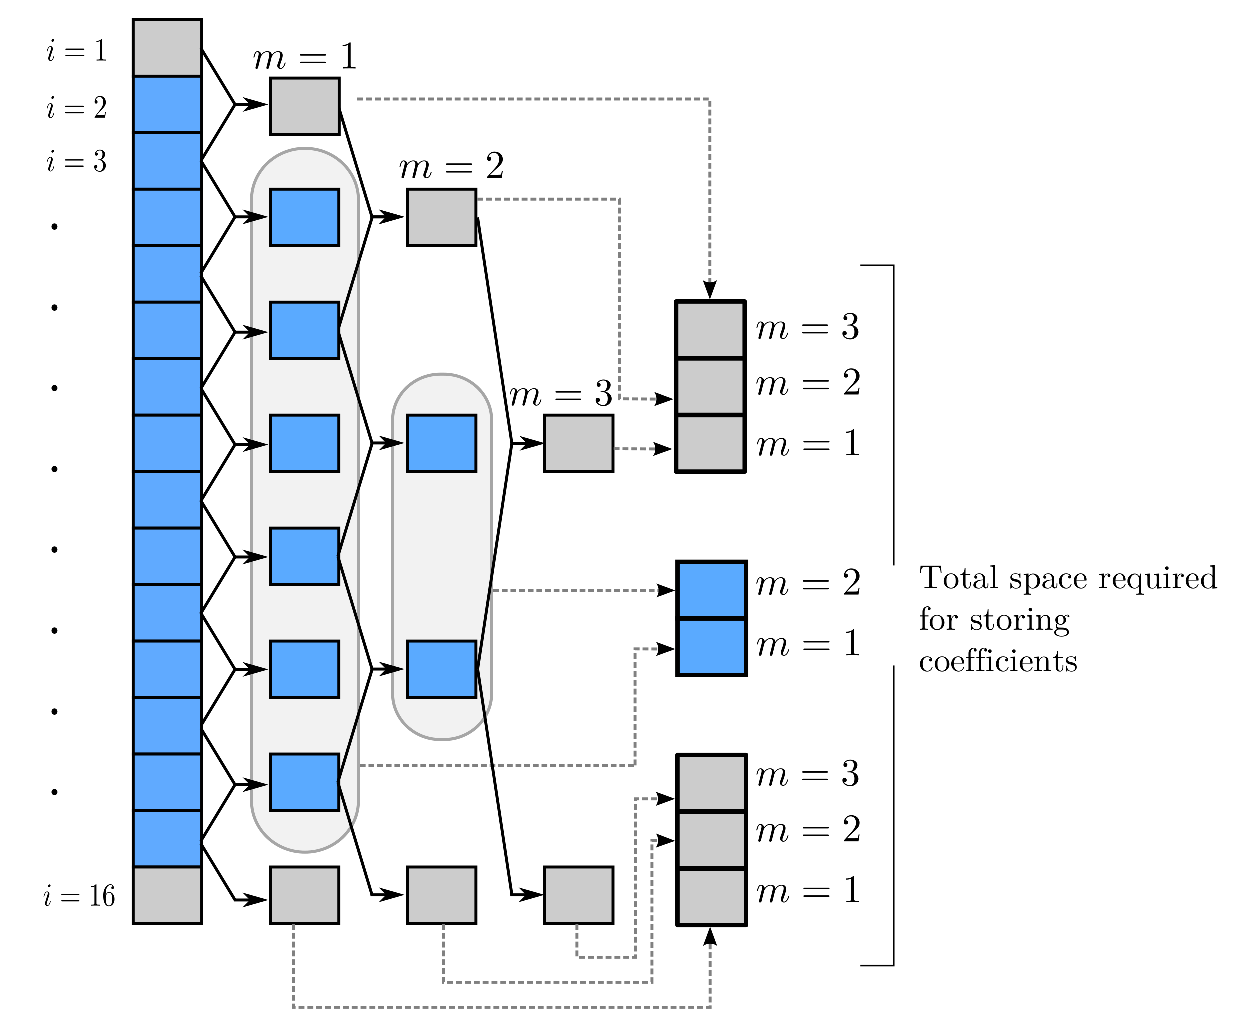
\includegraphics[height=200pt]{img/cyclic-reduction-precomputing.eps}
\end{center}
\caption{Maximum storage required for forward reduction coefficients
at all steps $m=1, 2, ... log_2(n)-1$}
\label{fig:cyclic-reduction-precomputing}
\end{figure}

Figure \ref{fig:cyclic-reduction-precomputing}
shows the
\emph{maximum} amount of storage required for
storing each of the coefficients
$\{b_1, c_1, a_0, b_0, c_0, a_n, b_n\}$,
or auxiliary variables $k_1$ and $k_2$.
A careful analysis of the
forward reduction and backward substitution equations
reveals that the actual amount of storage is somewhat less.
For instance,
the values $b_n^m$ are unused
in Eqs (\ref{eqn:precomputed-forward-reduction-step})-
(\ref{eqn:precomputed-backward-substitution-step-1}).
The values $a_n^m$ and $b_n^m$ are
required only for solving the $2-by-2$
system at the end of the forward reduction phase,
i.e., for $m=log_2(n)-1$,
and they are not stored for the previous steps.
Similarly, the values $c_1^m$ are equal to $c_0^m$,
and do not require special storage.
The set of precomputed coefficients required to be stored is then
$\{a_0^m, b_0^m, c_0^m, k_1^m, k_2^m, b_1^m, k_{1,1}^m, k_{1,n}^m\}$.
Each of these ``coefficient arrays'' are computed on the CPU
and transferred to the GPU.
Additionally, the two scalars $a_n^{log_2(n)-1}$ and $b_n^{log_2(n)-1}$
are required for the 2-by-2 solve.
%
\begin{figure}
\begin{center}
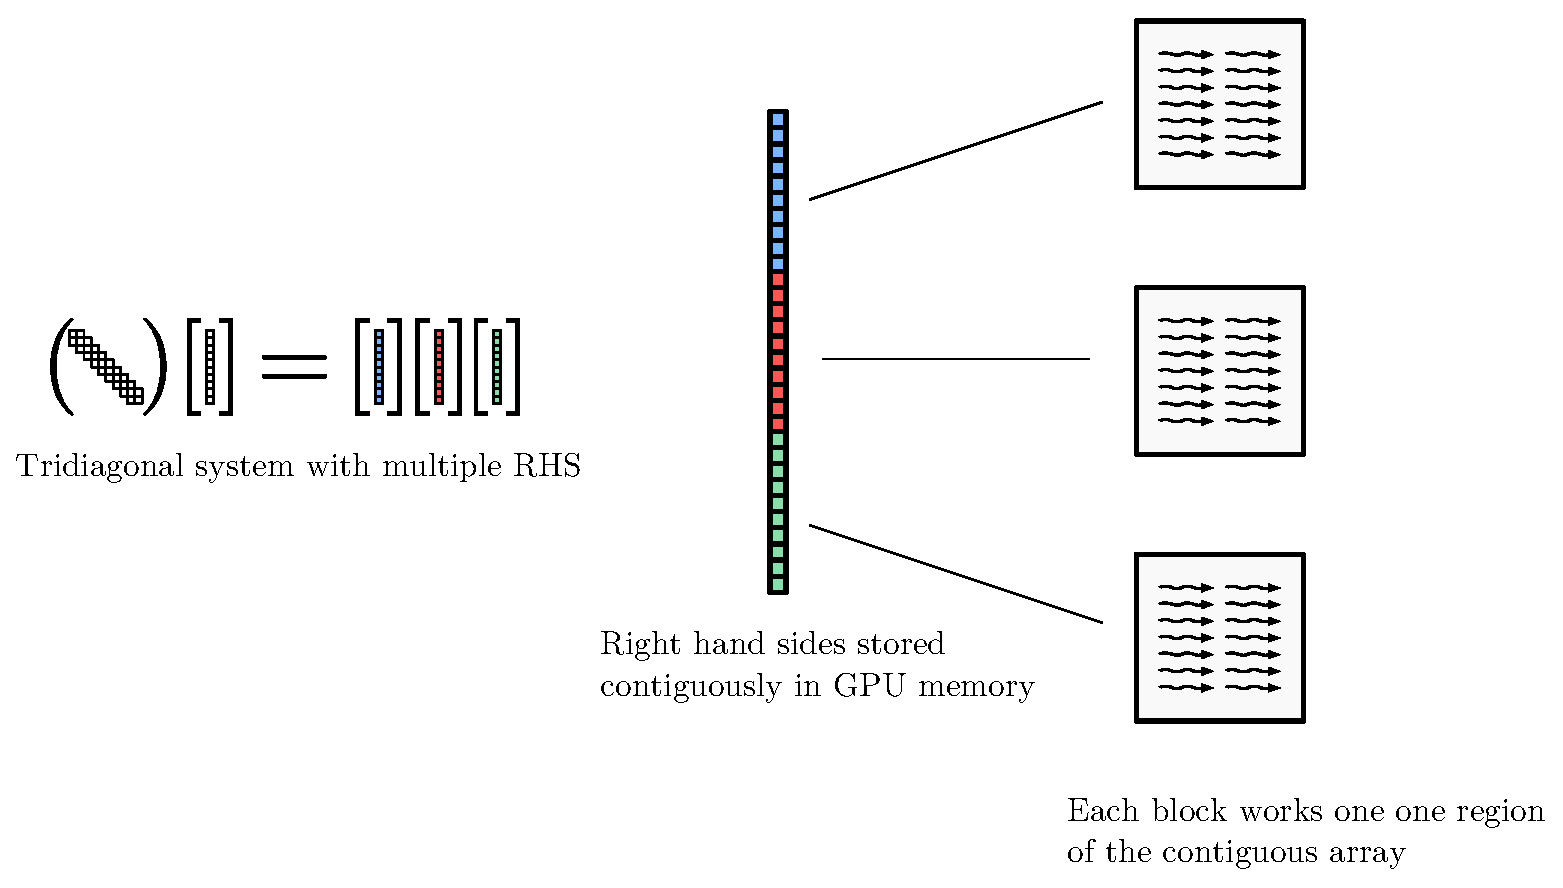
\includegraphics[height=200pt]{img/block-mapping.eps}
\end{center}
\caption{Storing right hand sides and mapping to thread blocks.}
\label{fig:block-mapping}
\end{figure}
%
The right hand sides that the system must be solved for
are stored in a single contiguous array in GPU memory
\ref{fig:block-mapping}.
The precomputed coefficient arrays and the right hand side array
are passed as inputs to the compute kernels that implement
the modified cyclic reduction.
We describe two implementations of the kernels,
the first works entirely with global memory,
and the second leverages the GPU's \emph{shared} memory.

\begin{figure}
\begin{center}
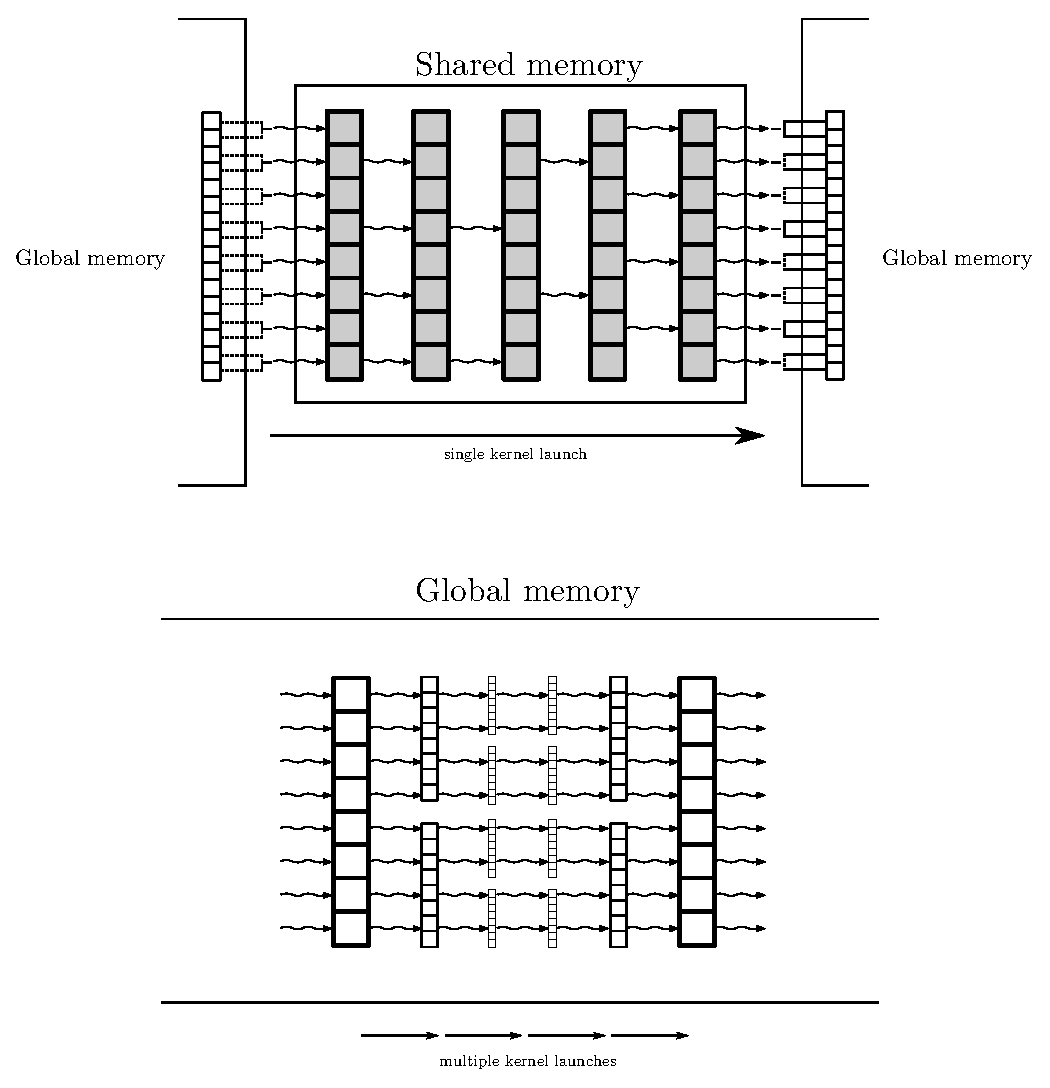
\includegraphics[width=400pt]{img/global-and-shared.eps}
\end{center}
\caption{Thread activity in shared memory (top) and global memory (bottom) implementations.}
\label{fig:global-and-shared}
\end{figure}

\subsection{Global memory implementation}

This implementation works entirely on the GPU's global memory,
Here, we define two kernels - one for the forward reduction step,
and the other for the backward substitution step.
Each kernel is called $log_2(n)-1$ times.
An extra call to the
forward reduction kernel performs
the two-by-two solve.
At each step,
the size of the thread blocks is determined by the \emph{stride}
between elements accessed at that step.
For the forward reduction phase,
we use $n/2$ threads per block for the first step,
$n/4$ threads for the second step, and so on.
The pattern is reversed for the backward substitution phase,
beginning with 2 threads per block for the first step.
Although this ensures that there are no inactive threads
at any stage,
the occupancy of the GPU is still very low
during the end of forward reduction and the end of backward substitution.
The precomputed coefficient arrays and right hand
are accessed by the kernels from global memory.
The kernel suffers from
strided memory access for the right-hand side,
but the precomputed coefficient values are accessed
without major coalescing problems.
Further, by precomputing the forward reduction coefficients,
we greatly reduce the number of computations
(and thus the number of uncoalesced memory accesses).

\subsection{Shared memory implementation}

In the shared memory approach (Fig. \ref{fig:global-and-shared}),
we launch a single kernel to perform the entire
cyclic reduction solve.
The kernel is launched with $n/2$ threads per block.
Each thread block is allocated a block of shared memory of size $n/2$.
Each thread of a block performs the first reduction step
[Eq. (\ref{eqn:precomputed-forward-reduction-step})]
by accessing the required values
$d_i$, $d_{i-1}$ and $d_{i+1}$ from global memory,
storing the result in shared memory.
In subsequent reduction steps,
$d_i$, $d_{i-1}$ and $d_{i+1}$
are accessed from shared memory,
avoiding the uncoalesced global memory accesses
seen in the global memory implementation.
In each back substitution step,
threads overwrite the existing values in shared memory
with the values of the solution.
In the final step,
shared memory is filled completely
with the even-indexed solution values.
Each thread then computes an odd-indexed solution value,
storing it directly in global memory
and copies the even-indexed solution value
from shared memory to global memory.
The entire solution is done in a single kernel launch
to hide the latency of
memory transfers between global and shared memory.
Explicit synchronization between the threads of a block
is required within the kernel at the end of each step.

The shared memory implementation suffers from two major issues:
first, the number of active threads is halved at each forward reduction step,
(and subsequently doubled at each backward reduction step).
Synchronization between threads of a block is necessary at each step.
Thus, a significant portion of the kernel execution time is
spent by idle threads waiting for active threads to complete execution.
Secondly, the strided access to the
right-hand side values leads to bank-conflicts.
However, the number of bank conflicts is significantly smaller
than in cyclic reduction implementations for general tridiagonal systems,
due the reduced number of computations performed.
